\documentclass[11pt]{article}
\usepackage{tikz}
\usetikzlibrary{scopes}
\usepackage{amsmath}
\usepackage[margin = 1.5in]{geometry}
%opening
\title{A Verification of Newton's Second Law of Motion}
\author{Andreas Badea}
\date{\today}


\begin{document}

\maketitle

\begin{center}
	\begin{tabular}{l r}
		Partner: & Matthew Kaminski \\ % Partner names
		Instructor: & Dr. Brad Miller % Instructor/supervisor
	\end{tabular}
\end{center}

\section{Introduction}
Isaac Newton's three laws of motion, first codified in his seminal \oldstylenums{1687} work \textit{Philosophi\ae{} Naturalis Principia Mathematica}, set the foundation for much of classical mechanics. The laws of motion describe the relationships between forces, velocity and acceleration. The second law in particular describes the resultant acceleration of a body given a force applied to that body. More precisely, it states, firstly, that the acceleration of a body undergone as a result of a given force is directly proportional to the net force applied to that body. Secondly, that the acceleration underwent is inversely proportional to the mass of the body. And finally, just so that we remember that we are, in fact, dealing with vector quantities, the direction of acceleration is the same direction as the net force on the body. All of these statements may be neatly and concisely summarized in the equation
 \begin{equation}
\vec{a} \propto \frac{\vec{F}}{m}. \label{EQ:1}
\end{equation}
In both the SI system of units and the US Customary system\footnote{In order for this to be true, one must be careful to use the appropriate units. If the slug is used as the unit of mass and the pound as the unit of force then the proportionality constant remains 1. Alternatively, one may also choose to use the pound as the unit of mass, in which case the poundal must be used as as the unit of force. In both cases the foot remains the base unit of length and the second the base unit of time}, the proportionality constant of this expression is just 1, allowing one to change the relationship to one of equality rather than proportionality. Additionally, with a simple bit of algebraic rearrangement we may rewrite the above equation \eqref{EQ:1} into the familiar form
\begin{equation}
\vec{F} = m \vec{a}.
\end{equation}
The above statement may be empirically verified by measuring the acceleration of a body of a certain mass undergoing a certain force and comparing the relationship of these values to the above statement. 
\section{Procedure}
In order to measure the relationship between these values, a small cart, the body which will undergo the acceleration, was placed on a flat tabletop. Attached to this cart was a string thats other end dangled of the edge of the table by way of a small pulley. On the end of the string, off the end of the table, a mass \(m\) lay attached by a small hook. In order to be able to vary the mass of the system another mass \(M\) rests on top of the cart. And in order to measure the distance the cart travels, and indirectly acceleration the car undergoes, an ultra sonic distance probe sits on the opposite end of the table.

\begin{figure}[h]
	\centering
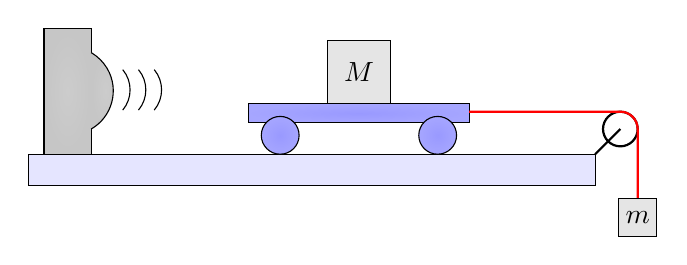
\begin{tikzpicture}
[scale = 8,
 plane/.style={draw=black,fill=blue!10},
 emit/.style={draw = black, inner color=lightgray!80 ,outer color=lightgray!90},
 cart/.style = {draw = black, inner color=blue!40,outer color=blue!35},
 mass/.style = {draw = black, fill = gray!20}
 ]
\draw [plane] (0.1,0) -- (1,0) -- (1,-0.05) -- (0.1,-0.05) -- (0.1,0);
\draw [emit] (0.125,0) rectangle (0.2,0.2);
\draw [emit] (0.2,0.04) arc (-60:60:0.07);
\draw (0.25,0.07) arc (-40:40:0.05);
\draw (0.3,0.07) arc (-40:40:0.05);
\draw (0.275,0.07) arc (-40:40:0.05);
\draw [cart] (0.45,0.05) rectangle ++ (0.35,0.03);
\draw [cart] (0.5,0.03) circle (0.03);
\draw [cart] (0.75,0.03) circle (0.03);
\draw [mass] (0.575,0.08) rectangle ++ (0.1,0.1) node[pos=.5] {\(M\)};
\draw [thick] (1.04,0.04) circle (0.0275);
\draw [thick] (1,0) -- (1.04,0.04);
\draw [red,thick] (0.8,0.0675) -- (1.04,0.0675) -- (1.04,0.0675) arc (90:0:0.0275) -- (1.0675,-0.1);
\draw [mass] (1.0675-0.03,-0.1-0.03) rectangle ++ (0.06,0.06) node[pos=.5] {\(m\)};
\end{tikzpicture}
\caption{The mass of \(m\) causes the cart and \(M\) to accelerate. }
\end{figure}

In order to avoid the movement of the cart prior to collection of data, the cart is held back by hand. Once collection of data has begun, the cart is allowed to move forward, and due to the weight of the mass \(m\), the cart begins to accelerate. Once the cart reaches a point close to the edge of the table, the cart is stopped and data collection ends.

Once the position data has been recorded, its first derivative with respect to time is taken numerically. This represents the velocity of the cart at a given time. The portion of time, in which the velocity appears to be linear is the portion of time that the cart is accelerating due to the weight of \(m\). The slope of this is recorded and deemed to be the acceleration experience by the system during the time of interest.

\section{Data}
\section{Analysis}
\section{Results and Conclusions}

\end{document}